%% Source Template:
%% Copyright (C) 2014 by Pascal Richter, Elena Botoeva, Richard Barnard, and Dirk Surmann
%% 
%% This file may be distributed and/or modified under the
%% conditions of the LaTeX Project Public License, either
%% version 2.0 of this license or (at your option) any later
%% version. The latest version of this license is in:
%% 
%% http://www.latex-project.org/lppl.txt
%% 
%% and version 2.0 or later is part of all distributions of
%% LaTeX version 2013/12/01 or later.
%% 

\documentclass[20pt, a1paper, portrait, margin=0mm, innermargin=15mm]{tikzposter} %Options for format can be included here

% Header
\title{Gravitational waves from Neutron stars}
\author{Gregory Ashton, Supervised by D.I. Jones \& R. Prix }
\institute{University of Southampton}
%\titlegraphic{LogoGraphic Inserted Here}

 %Choose Layout
\usetheme{Autumn}

% Additonal packages
\usepackage{wrapfig}
\usepackage{multicol}

\begin{document}

 % Title block with title, author, logo, etc.
\maketitle


 \block{Introduction}{

}


 \begin{columns}

 % FIRST column
\column{0.5}

\block[]{What is a \emph{gravitational wave}?}{
Einstein formulated general relativity in 1916, like all good theories
it made several important predictions. All but one of these have been
tested and agree with the theory. The final prediction of GW that we want 
to directly observe is \emph{gravitational waves}. 
\begin{wrapfigure}[5]{l}{0.4\linewidth}
\begin{tikzfigure}
\centering

\includegraphics[width=0.8\linewidth]{img/star_with_GW-crop}
\end{tikzfigure}
\end{wrapfigure}
Einstein unified the ideas of space and time into a single object \emph{spacetime}.
Spacetime is a dynamic object that can be curved, picture it like a stretched rubber
sheet. Large masses can curve the space time, this is like placing weights on the
rubber sheet. But this picture can evolve in time we say that:
\emph{ spacetime tells matter how to much while matter tells spacetime how to curve.}
Gravitational waves can result from the rotation of a massive mass that isn't
perfectly symmetric. They are ripples in spacetime literally ..
}

 % SECOND column
\column{0.5}

\block{What is a \emph{neutron star}?}{

Stars like our sun are in an equilibrium between the outward force from
burning nuclear fuel in their core and collapse due to their own gravity.
\begin{wrapfigure}{r}{0.4\linewidth}
\begin{tikzfigure}
\centering
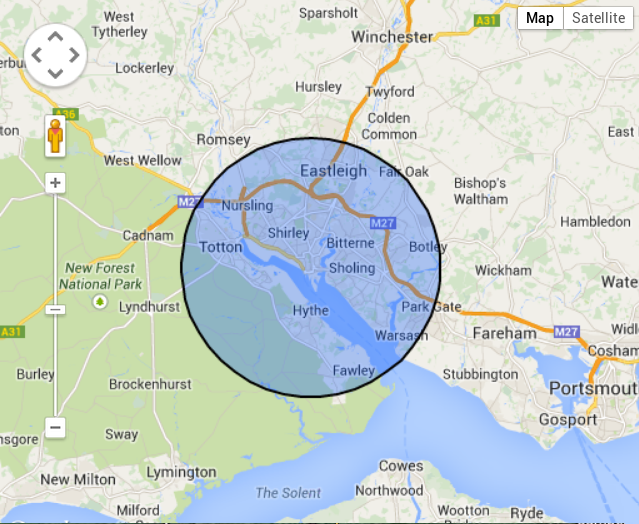
\includegraphics[width=0.9\linewidth]{img/southampton}
\end{tikzfigure}
\end{wrapfigure}
When they run out of fuel they collapse, some of them collapse to form a
neutron star. 
These are extremely dense: they have a mass about that of our sun but are only 10km across 
a typical diameter is compared to Southampton in the image on the right.

\begin{wrapfigure}{l}{0.5\linewidth}
\begin{tikzfigure}
\centering
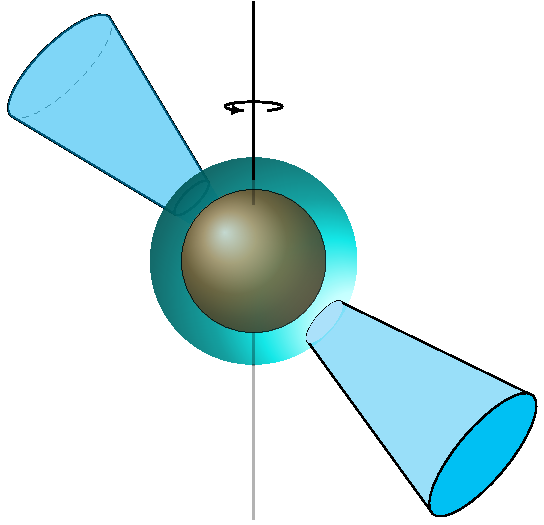
\includegraphics[width=0.9\linewidth]{img/star-crop}
\end{tikzfigure}
\end{wrapfigure}
We see some neutron stars as pulses of electromagnetic light. This is caused
by radiation streaming out in thin beams passing over the earth like a lighthouse. 

Neutron stars contain lots of interesting physics such as massive magnetic fields
and exotic forms of matter. For us though, the most interesting thing is that
they may emit gravitational waves. 
}

\end{columns}

\block[]{Searching for gravitational waves from neutron stars}{
\begin{multicols}{3}
\begin{tikzfigure}[LIGO]
\centering
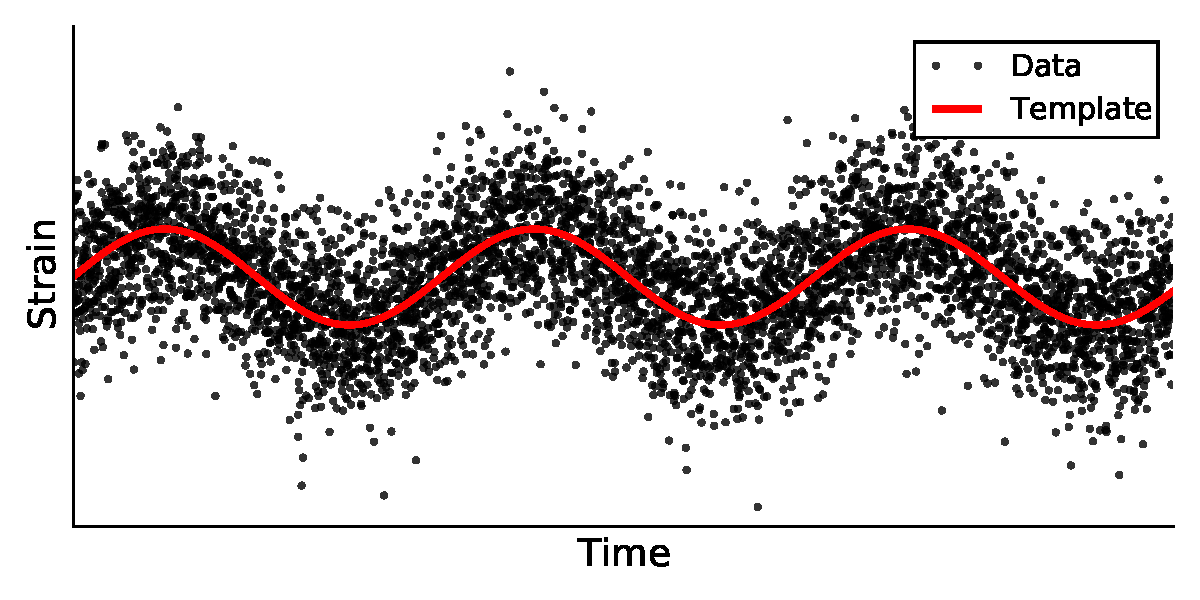
\includegraphics[width=1.0\linewidth]{img/CGW_example}
\end{tikzfigure}
\columnbreak
To search for GWs we use laser interferometers 

\columnbreak

\begin{tikzfigure}[LIGO]
\centering
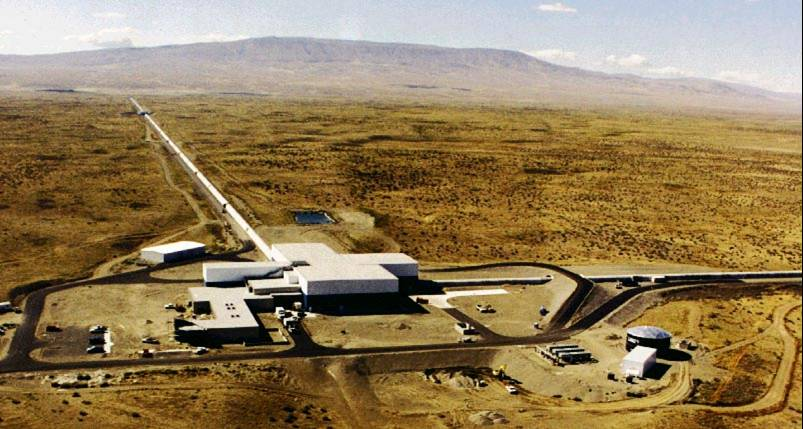
\includegraphics[width=1.0\linewidth]{img/Hanford1}
\end{tikzfigure}


\end{multicols}
}

\block[]{Timing noise from neutron stars}{}

\block[]{Conclusions}{}

\end{document}



\endinput
%%
%% End of file `tikzposter-template.tex'.
